\documentclass[12pt]{article}
\usepackage[a4paper, margin=1in]{geometry}
\usepackage{enumitem}
\usepackage{titlesec}
\usepackage{graphicx}
\usepackage{hyperref}
\usepackage{float}

\titleformat{\section}{\Large\bfseries}{\thesection}{1em}{}
\titleformat{\subsection}{\large\bfseries}{\thesubsection}{1em}{}

\title{Architectural Requirements\\Taxi Tap by Git It Done}
\date{}

\begin{document}

\maketitle

\begin{figure}[H]
  \centering
  
\includegraphics[width=0.5\textwidth]{LogoGroup.png} 
\end{figure}

\begin{figure}[H]
  \centering
  
\includegraphics[width=0.5\textwidth]{LogoTaxiTap.png} 
\end{figure}

\newpage

\tableofcontents
\newpage

\section{Introduction}

TaxiTap is a comprehensive taxi booking and management application designed to connect passengers with drivers in real-time. The system provides a seamless, secure, and scalable solution for urban transportation needs. This document outlines the architectural decisions, quality requirements, and technical strategies employed to deliver a robust, high-performance mobile application.
The system facilitates ride booking, real-time tracking, and driver management through an intuitive mobile interface backed by a serverless architecture.

\section{Architectural Design Strategy}

\textbf{Strategy Chosen:} \textit{Decomposition via Feature-Driven Development (FDD)}

TaxiTap is built using a modular, feature-based decomposition strategy that aligns with our quality requirements of availability, scalability, and usability. Each functional system (e.g., User System, Vehicle System, Trip System) is designed, tested, and deployed independently.

Benefits of this strategy:

\begin{itemize}
  \item Clear modularity: Separation of concerns enables focused development and maintenance.
  \item Parallel development: Multiple features can be developed simultaneously by different team members.
  \item Changes to one feature have minimal impact on others
  \item Scalability: Features can be scaled based on demand without affecting the entire system
  \item Reduced risk: Changes to one feature have minimal impact on others.
\end{itemize}

This strategy was chosen because it directly supports our top three quality requirements:

\begin{itemize}
\item Availability - Failure in one module doesn't bring down the entire system
\item Scalability - Individual modules can be scaled independently
\item Usability - Clear feature boundaries lead to better user experience design
\end{itemize}

\section{Architectural Strategies}
\textbf{Chosen Style:} \textit{Event-Driven Architecture}

Event-driven architecture is centered around asynchronous communication between components. Components emit and react to events, allowing for real-time responsiveness, loose coupling and scalability.
Why this is the best fit for our system:

\begin{itemize}
  \item Real-time Interaction: Location updates, ride requests, driver availability, and notifications all benefit from real-time triggers and updates. Convex supports reactive data and background functions, making it a natural fit for an event-driven model.
  \item Asynchronous Processing: Tasks like sending push notifications, updating seat availability, or logging analytics should not block the main user flow. EDA allows these to run in the background, improving app responsiveness.
  \item Loose Coupling: With EDA, components (like driver matching and notifications) can be developed and deployed independently. This aligns well with Convex’s function-based model, which is modular and reactive.
  \item Scalability and Maintainability: New features can easily be added by listening to events without modifying core components.
\end{itemize}

\subsection{Architectural Strategies extended}
\begin{itemize}
  \item \textbf{Availability:} \\
  \textbf{Problem:} If the system becomes unavailable, users cannot book or accept rides, damaging both reliability and trust. \\
  \textbf{Solution:} 
  \begin{itemize}
    \item \textbf{Replication:} Convex provides high availability by replicating data and functions across multiple geographic zones, ensuring continuity during failures.
  \end{itemize}
  
  \item \textbf{Scalability:} \\
  \textbf{Problem:} To support growing demand and simultaneous ride requests, the system must dynamically handle increased load. \\
  \textbf{Solution:} 
  \begin{itemize}
    \item \textbf{Horizontal scale-out:} Convex automatically scales infrastructure horizontally to meet demand. Convex handles horizontal scaling of function execution through a service called Funrun. This service allows for the distribution of function execution across multiple machines, enabling a more scalable and performant system.
    \item \textbf{Data sharding:} Data is partitioned across shards by Convex without manual configuration, improving scalability. Convex handles data sharding primarily through Components and Sharded Counters. Components, like the Sharded Counter, are isolated units of logic that handle specific tasks and provide transactional consistency, even when dealing with potentially conflicting operations.
    \item \textbf{Asynchronous processing:} Non-critical tasks (e.g., sending notifications) are offloaded to background jobs using Convex async functions, freeing up system resources.
  \end{itemize}

  \item \textbf{Usability:} \\
  \textbf{Problem:} An intuitive and responsive interface is crucial to support users with varying levels of digital literacy. \\
  \textbf{Solution:} 
  \begin{itemize}
    \item \textbf{Real-time UI:} Keeps location and notification data live using subscriptions or efficient polling mechanisms.
    \item \textbf{Responsiveness:} Improves user experience by minimizing UI latency and limiting the use of loading spinners to essential operations.
  \end{itemize}

  \item \textbf{Security:} \\
  \textbf{Problem:} The system manages sensitive user data, including real-time locations and account details. Breaches can result in legal and reputational harm. \\
  \textbf{Solution:} 
  \begin{itemize}
    \item \textbf{Secure communication:} All data in transit is encrypted using TLS by default.
    \item \textbf{Role-based access control (RBAC):} Server functions enforce strict access controls based on user roles (e.g., driver vs passenger).
  \end{itemize}

  \item \textbf{Performance:} \\
  \textbf{Problem:} Real-time systems require fast responses. Delays in booking, tracking, or communication reduce system usability. \\
  \textbf{Solution:} 
  \begin{itemize}
    \item \textbf{Database indexing:} Convex uses optimized queries with \texttt{withIndex(...)} for fast access to common fields like driver ID or ride ID.
    \item \textbf{Asynchronous tasks:} Operations like sending notifications are processed asynchronously to reduce response time for users.
  \end{itemize}
\end{itemize}

\section{Architectural Quality Requirements}
\subsection{Quality attributes}
The following quality requirements are prioritized based on client needs and system criticality:

\begin{itemize}
  \item \textbf{Availability:} \\
  \textbf{Why it's a top quality requirement:} Ensures continuous service. If the app is down, users cannot book or accept rides, which impacts revenue and reputation. \\

\begin{table}[H]
\centering
\begin{tabular}{|l|p{10cm}|}
\hline
\textbf{Stimulus Source} & System failures, network issues, or high load \\
\hline
\textbf{Stimulus} & System components become unavailable or unresponsive \\
\hline
\textbf{Response} & System maintains service continuity with graceful degradation \\
\hline
\textbf{Response Measure} & 
\begin{itemize}
  \item 99.5\% uptime under normal usage
  % \item Automatic failover within 30 seconds
  % \item Service restoration within 2 minutes
\end{itemize} \\
\hline
\textbf{Environment} & Normal and peak operating conditions \\
\hline
\textbf{Artifact} & Entire system infrastructure including database and backend \\
\hline
\end{tabular}
\end{table}
  
  \item \textbf{Scalability:} \\
  \textbf{Why it's a top quality requirement:} Supports many users using the app simultaneously and allows the system to handle growth in demand. \\

  \begin{table}[H]
\centering
\begin{tabular}{|l|p{10cm}|}
\hline
\textbf{Stimulus Source} & Increasing user base and concurrent ride requests \\
\hline
\textbf{Stimulus} & System must handle growing demand without performance degradation \\
\hline
\textbf{Response} & Horizontal scaling of services and database sharding \\
\hline
\textbf{Response Measure} & 
\begin{itemize}
  \item Support 100+ concurrent ride requests
  \item Maintain response times under increased load
  \item Auto-scale infrastructure based on demand
\end{itemize} \\
\hline
\textbf{Environment} & Variable load conditions from low to peak usage \\
\hline
\textbf{Artifact} & Backend services, database, and infrastructure \\
\hline
\end{tabular}
\end{table}

  \item \textbf{Usability:} \\
  \textbf{Why it's a top quality requirement:} Users must be able to complete essential tasks easily, regardless of their technical skill level. Poor usability leads to frustration and abandonment. \\

\begin{table}[H]
\centering
\begin{tabular}{|l|p{10cm}|}
\hline
\textbf{Stimulus Source} & Users with varying technical skills using the app \\
\hline
\textbf{Stimulus} & Users need to complete ride booking and payment tasks easily \\
\hline
\textbf{Response} & Use simple language, clear layout, and high-contrast color schemes. Employ interface metaphors such as intuitive icons to make navigation easy for users, including those who are technologically inexperienced \\
\hline
\textbf{Response Measure} & 
\begin{itemize}
  \item Task completion within a few clicks
  % \item 70\%+ user satisfaction rating
  % \item 5-minute learning curve for new users
\end{itemize} \\
\hline
\textbf{Environment} & Mobile device usage in various conditions \\
\hline
\textbf{Artifact} & User interface, navigation flow, visual design \\
\hline
\end{tabular}
\end{table}

  \item \textbf{Security:} \\
  \textbf{Why it's a top quality requirement:} The system manages sensitive user data, including locations and contact details. Breaches can result in legal issues and loss of trust. \\

  \begin{table}[H]
\centering
\begin{tabular}{|l|p{10cm}|}
\hline
\textbf{Stimulus Source} & Unauthorized access attempts or data breaches \\
\hline
\textbf{Stimulus} & Users/attackers attempting to access sensitive data \\
\hline
\textbf{Response} & System enforces strict access controls and data protection \\
\hline
\textbf{Response Measure} & 
\begin{itemize}
  \item Role-based access control (RBAC) enforced
  \item Data encrypted in transit and at rest
  \item Authentication tokens validated
\end{itemize} \\
\hline
\textbf{Environment} & All system interactions and data access \\
\hline
\textbf{Artifact} & User data, location information, payment details \\
\hline
\end{tabular}
\end{table}

  \item \textbf{Performance:} \\
  \textbf{Why it's a top quality requirement:} Real-time features must respond quickly to meet user expectations. Delays in booking, navigation, or messaging reduce usability during peak hours. \\

  \begin{table}[H]
\centering
\begin{tabular}{|l|p{10cm}|}
\hline
\textbf{Stimulus Source} & User/Driver requesting ride booking or location updates \\
\hline
\textbf{Stimulus} & User wants real-time responses for booking, tracking, and navigation \\
\hline
\textbf{Response} & System provides immediate feedback and updates \\
\hline
\textbf{Response Measure} & 
\begin{itemize}
  \item Backend functions respond within 20ms average
  \item Location updates occur every time the user moves
  \item Ride requests processed within 100ms
\end{itemize} \\
\hline
\textbf{Environment} & Peak usage hours with high concurrent users \\
\hline
\textbf{Artifact} & Mobile app, backend functions, database queries \\
\hline
\end{tabular}
\end{table}
\end{itemize}

\section{Architectural Patterns}

This section discusses the key architectural patterns employed in our system, along with their motivations, the quality requirements they support, and their specific application in our implementation.

\subsection{Leader-Follower (Replication)}

\textbf{Purpose:} The Leader-Follower pattern replicates services or data across nodes to ensure availability and failover.

\textbf{Why We Use It:} To provide high availability and data redundancy. In case one instance fails, another replica can take over.

\textbf{Quality Requirement Supported:}
\begin{itemize}
    \item \textbf{Availability}
\end{itemize}

\textbf{Application in System:}  
Convex’s serverless backend infrastructure employs automatic replication of data and functions across multiple zones. This ensures continued access to services even if a zone experiences downtime. It also supports strong consistency guarantees without requiring developers to manage replicas manually.

\subsection{Service-Oriented Architecture}

\textbf{Purpose:}  
To structure the system as a set of loosely coupled, reusable services that communicate over well-defined interfaces. Each service encapsulates a specific business capability, enabling flexibility in deployment and evolution.

\textbf{Why We Use It:}  
Taxi Tap uses SOA to separate key business functions—such as ride booking, driver management, payment processing, and notifications—into independent services. This allows teams to develop, maintain, and deploy each service without impacting others, while still integrating them into a cohesive platform through standard service contracts.

\textbf{Quality Requirements Supported:}  
\begin{itemize}
  \item \textbf{Scalability} – Services can scale independently depending on load. For example, the ride booking service can be scaled up during peak hours without affecting payment processing.
  \item \textbf{Performance} – Limits cross-service interference; e.g., high load on the booking service does not slow down authentication or driver location tracking.
\end{itemize}

\textbf{Application in System:}  
In Taxi Tap, the SOA approach ensures that each core function (e.g., Booking Service, Authentication Service, Payment Service, Location Service) operates as an independent service. These services communicate via a defined API, enabling the system to replace or update services without a full system redeployment. For example, the Payment Service manages transaction records independently from the Ride Service's booking data, connected only through shared ride identifiers.

\subsection{Event-Driven Architecture}

\textbf{Purpose:} Decouple services by communicating through asynchronous events.

\textbf{Why We Use It:} To handle asynchronous workflows, reduce coupling, and improve responsiveness under load.

\textbf{Quality Requirements Supported:}
\begin{itemize}
  \item \textbf{Scalability} – Events allow services to scale independently.
  \item \textbf{Performance} – Asynchronous processing ensures quick responses.
  \item \textbf{Availability} – Temporary service disruptions don't block upstream operations.
\end{itemize}

\textbf{Application in System:}  
Convex background functions are used to handle side effects such as updating ride history, sending notifications, and recalculating driver ratings. These tasks are decoupled from the main user actions (e.g., booking a ride), improving perceived responsiveness. Events like \texttt{rideRequested}, \texttt{rideCompleted}, and \texttt{locationUpdated} are used to trigger background logic.

\subsection{Model-View-ViewModel (MVVM)}

\textbf{Purpose:} Promote separation of concerns between UI, state, and business logic.

\textbf{Why We Use It:} To create maintainable and testable frontend code, and to simplify UI state synchronization.

\textbf{Quality Requirement Supported:} 
\begin{itemize}
   \item \textbf{Usability}
\end{itemize}  

\textbf{Application in System:}  
Frontend components (built using React Native) follow MVVM principles:
\begin{itemize}
  \item \textbf{Model:} Convex queries and mutations represent data.
  \item \textbf{ViewModel:} Hooks like \texttt{useQuery}, \texttt{useState}, and custom context (e.g., \texttt{ThemeContext}) manage UI logic.
  \item \textbf{View:} React components render based on ViewModel state.
\end{itemize}
This enables real-time updates (e.g. seat availability or route filtering) with a clean separation of concerns, enhancing user experience.

\section{Design patterns}

\paragraph{Observer Pattern}

\begin{itemize}
    \item Pattern Type: Behavioural
    \item Participants:
    \begin{itemize}
        \item Subject: Notification System
        \item Observer: User
        \item Concrete Observer: Passenger, Driver 
    \end{itemize}
    \item Explanation: The Observer pattern allows an object (User) to be notified automatically of state changes in another object (Notification System). This is ideal for handling events like route updates or ride status.
    \item Example:
    \begin{itemize}
        \item User receives alerts from the Notification System.
        \item Notification System initiates a notification when a route is announced.
    \end{itemize}
\end{itemize}

\paragraph{Mediator Pattern}

\begin{itemize}
    \item Pattern Type: Behavioural
    \item Participants:
    \begin{itemize}
        \item Mediator: Taxi Request System
        \item Colleague: Passenger, Driver
    \end{itemize}
    \item Explanation: The Mediator pattern centralizes complex communication between objects. Instead of Passenger directly interacting with Driver, requests are handled through the Taxi Request System.
    \item Example:
    \begin{itemize}
        \item Taxi Request System acts as an intermediary between Passenger and Driver.
        \item Passenger makes a request for pickup to a driver, but the Taxi request system acts as the middleman for this request.
    \end{itemize}
\end{itemize}

\section{Architectural Design}
\textbf{Overview:} Taxi Tap is structured using a feature-driven and event-driven architecture. The diagram below illustrates this architecture.

\vspace{1em}
\begin{figure}[H]
  \centering
  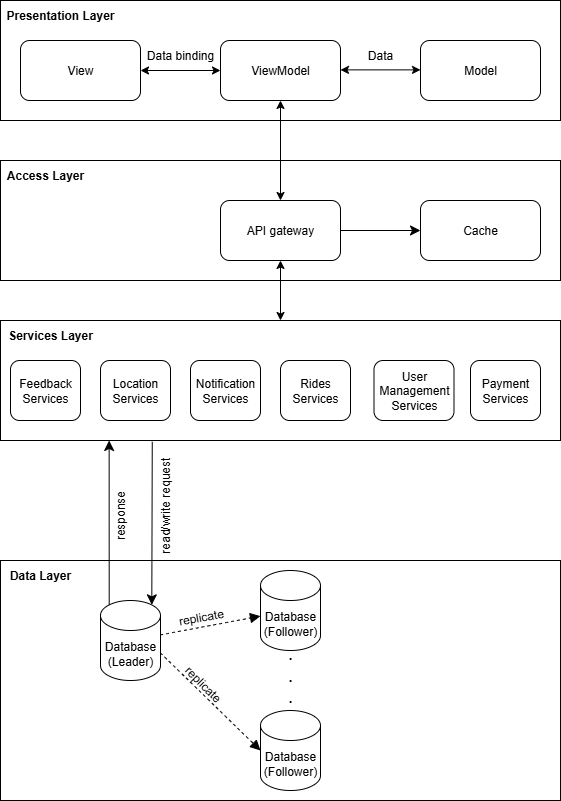
\includegraphics[width=1\textwidth]{Architecural Diagram.png}
  \caption{Architecture Diagram}
\end{figure}

\textbf{Components:}

\begin{itemize}
  \item \textbf{Expo Frontend:} Mobile-first interface using React Native. The user intefraces are built with MVVM.
  \item \textbf{Convex Backend:} Serverless backend with modular mutations and schema.
  \item \textbf{Convex Database:} Strongly-typed database used by each module.
\end{itemize}

This design provides modularity, scalability, and testability with minimal DevOps complexity.

\section{Architectural Constraints}
\begin{itemize}
  \item \textbf{Client Constraints:} Must remain within the AWS Free Tier; performance must be maintained under low-cost infrastructure.
  \item \textbf{Deployment Constraints:} Fully serverless; no Docker/Kubernetes; must deploy via CI/CD with minimal setup.
  \item \textbf{Security Constraints:} Only verified users may access trip, payment, or GPS functionality.
  \item \textbf{Latency Constraints:} Real-time location updates must occur.
  \item \textbf{Scalability Constraints:} Design must accommodate scaling to 1,000+ users without architectural changes.
\end{itemize}

\section{Technology Choices}

\subsubsection*{Backend Platform}
\begin{tabular}{|l|p{6cm}|p{6cm}|}
\hline
\textbf{Option} & \textbf{Pros} & \textbf{Cons} \\
\hline
Convex & Fully serverless, fast dev, native React support & New ecosystem, TypeScript only \\
\hline
Firebase & Realtime syncing, easy integration & Poor test tooling, security rule complexity \\
\hline
AWS Lambda & Highly scalable, mature & Complex CI/CD, requires DevOps setup \\
\hline
\textbf{Chosen:} Convex & \multicolumn{2}{l|}{Perfect fit for modular, testable architecture. Free tier-friendly.} \\
\hline
\end{tabular}

\vspace{1em}

\subsubsection*{Frontend Platform}
\begin{tabular}{|l|p{6cm}|p{6cm}|}
\hline
\textbf{Option} & \textbf{Pros} & \textbf{Cons} \\
\hline
Expo (React Native) & Fast prototyping, hot reload, cross-platform & Slightly heavier bundles \\
\hline
Flutter & Beautiful UI, good performance & Slower iteration, Dart-only \\
\hline
Native iOS/Android & Highest performance & High dev effort, no code sharing \\
\hline
\textbf{Chosen:} Expo & \multicolumn{2}{l|}{Fastest mobile-first path with TypeScript and Convex integration.} \\
\hline
\end{tabular}

\vspace{1em}

\subsubsection*{Database}
\begin{tabular}{|l|p{6cm}|p{6cm}|}
\hline
\textbf{Option} & \textbf{Pros} & \textbf{Cons} \\
\hline
Convex DB & Type-safe, built for Convex, no config & Smaller community \\
\hline
Firestore & Realtime, battle-tested & Complex security model \\
\hline
Supabase & Postgres-based, open source & Overhead for micro-systems \\
\hline
\textbf{Chosen:} Convex DB & \multicolumn{2}{l|}{Natively integrated with our serverless logic.} \\
\hline
\end{tabular}

\section{Deployment Model}
The system will be deployed following a cloud-based deployment model to ensure scalability, availability, and ease of access. The deployment environment will include:
\begin{itemize}
    \item \textbf{Frontend:} Deployed via Expo Go.
    \item \textbf{Backend:} Hosted on Convex cloud (Convex backend as a service).
    \item \textbf{Database:}  Managed by Convex (integrated serverless database).
    \item \textbf{CI/CD:} Managed via GitHub Actions to automate linting, testing and deployment.
\end{itemize}

The system is deployed using a cloud-based deployment model. The deployment pipeline follows a CI/CD workflow that integrates development, continuous integration, and continuous deployment. During development, source code is managed through GitHub, with developers using Expo Go for mobile app testing and Convex Dev for backend testing in a local environment. Once changes are committed and pushed to GitHub, the CI pipeline is triggered via GitHub Actions, where automated steps such as linting, formatting, and testing are executed to ensure code quality and consistency. After successful integration, the CD pipeline automatically deploys the validated build to the target production environment hosted in the Convex cloud platform. The deployment topology follows a multi-tier architecture, where the frontend (mobile client) communicates with backend services hosted in Convex, which provides serverless functions, database storage, and scaling capabilities. The diagram illustrates this process, showing the transition from local development through GitHub-based integration pipelines to final deployment in Convex Production.

\begin{figure}[H]
  \centering
  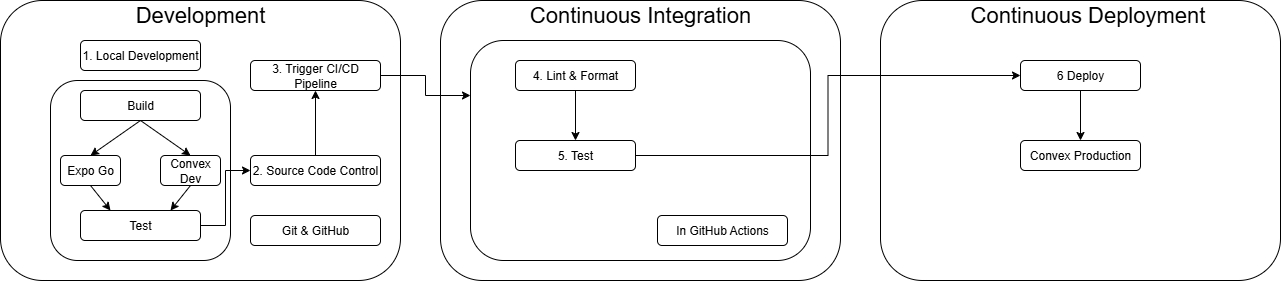
\includegraphics[width=1\textwidth]{Deployment Model.png}
  \caption{Deployment Diagram}
\end{figure}

\section{Live Deployed System}
A fully functional live version of the system will be accessible for demonstration purposes. This deployed system will allow real-time interaction by both drivers and passengers via mobile devices. The system will include:
\begin{itemize}
    \item User registration and authentication.
    \item Route selection and ride request.
    \item Real-time updates.
    \item Feedback and rating system.
    \item User account management.
    \item Cash payment support.
\end{itemize}

\end{document}